\section{Probability Recap, Loss Functions, Logistic Regression, Neural Networks Intro}
\subsection{Probability Basics}
\textbf{Random Variable (RV)} \(x\) denotes a quatity that is uncertain, discret or continuous.
\(p(x = \mathbb{X})\): the probability of variable \(x\) being in state \(\mathbb{X}\).

\textbf{Domain of RV} denotes all the values it can take (states it can be in).
\(\text{dom}(coin) = \{\text{heads,tails}\}\)


\textbf{Joint distribution} of two RVs \(x\) and \(y\) takes a particular combination of values and the joint probability density satisfies:
\[
\int\int Pr(x,y) \cdot dxdy = 1
\]

\textbf{Marginal distributions} \(Pr(x)\) and \(Pr(y)\) are obtained by:
\[
    \int\ Pr(x,y) \cdot dx = Pr(y)
\]
\[
    \int\ Pr(x,y) \cdot dy = Pr(x)
\]

Conditional probability \(Pr(x|y)\) is the probability of a variable \(x\) taking a certain value assuming we know the value of \(y\):
\[
Pr(x|y) = \frac{Pr(x,y)}{Pr(y)}
\]

\subsubsection{probability rules}
Sum rule:
\[
p(X) = \sum_{Y}p(X,Y)
\]
Product rule:
\[
p(X,Y) = p(Y|X) \cdot p(X) = p(X|Y) \cdot p(Y)
\]
Bayes Theorem:
\[
p(Y|X) = \frac{p(X|Y)\cdot p(Y)}{p(X)} = \frac{p(X|Y)\cdot p(Y)}{\sum_{y \in Y}p(X,y)} = \frac{p(X|Y)\cdot p(Y)}{\sum_{y}p(X,y)\cdot p(y)}
\]
\subsubsection*{Probability distributions and PDFs}
\[
\mathbb{E}\left[x\right] = \mathbb{E}_{x \sim p}\left[x\right] = \int x \cdot p(x)\,dx = \mu
\]
\[
\mathbb{E}\left[x^2\right] = \mathbb{E}_{x \sim p}\left[x^2\right] = \int x^2 \cdot p(x)\,dx = \mu^2 + \sigma^2
\]
\[
\mathbf{VAR}\left[x\right] = \mathbb{E}\left[x^2\right] - \mathbb{E}\left[x\right] = \sigma^2
\]
\subsection{Designing Loss Functions}
Loss/cost function measures how bad the model is - the lower the value of the loss function the better the model maps inputs to output \(\hat{\phi} = \arg\min\left[\text{L}[\phi]\right]\).

Model training is finding parameter values that minimize the loss.

The negative log likelihood (to be minimized) gives us a loss function.
\[
\hat{\phi} = \arg\min_\phi\left[-\sum_{i = 1}^{I}\log\left[Pr(y_i|f(x_i,\phi))\right]\right]
\]
\subsection{Logistic Regression}
Binary classification.
Output is the probability that the input belongs to a class.
\[
y = \text{logistic}(\mathbf{w}^T\mathbf{x}) = \frac{1}{1 + e^{-\mathbf{w}^T\mathbf{x}}}
\]
\subsubsection{Loss function (Binary Cross Entropy Loss)}
\[
J(\theta) = -\frac{1}{N}\sum_{i = 1}^{N}\left[y_i \log\hat{y_i}+  (1-y_i)\log(1-\hat{y_i})\right]
\]
Leads to the following update rule:
\[
\theta_j = \theta_j - \alpha\frac{\partial J(\theta)}{\partial \theta_j}
\]
this is simplified to:
\[
    \theta_j = \theta_j - \alpha\frac{1}{N}\sum_{i = 1}^{N}(\hat{y_i}-y_i)x^{(j)}_i
\]

\subsection{Neural Networks Basics}
Neural Networks (NN) consist of Neurons.
The value of a Neuron is defined by its connections to tha last layer, the weights(\(w_i\)) of the connection, the bias(\(b\)) and the activation funtion of the Neuron.
\begin{figure}[!h]
    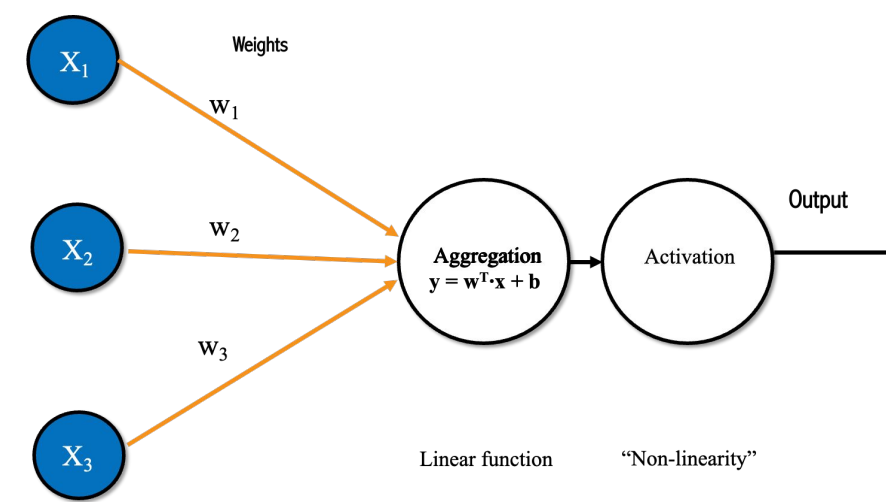
\includegraphics[width = \columnwidth]{figures/05/Neuron.png}
\end{figure}
\begin{figure}[!h]
    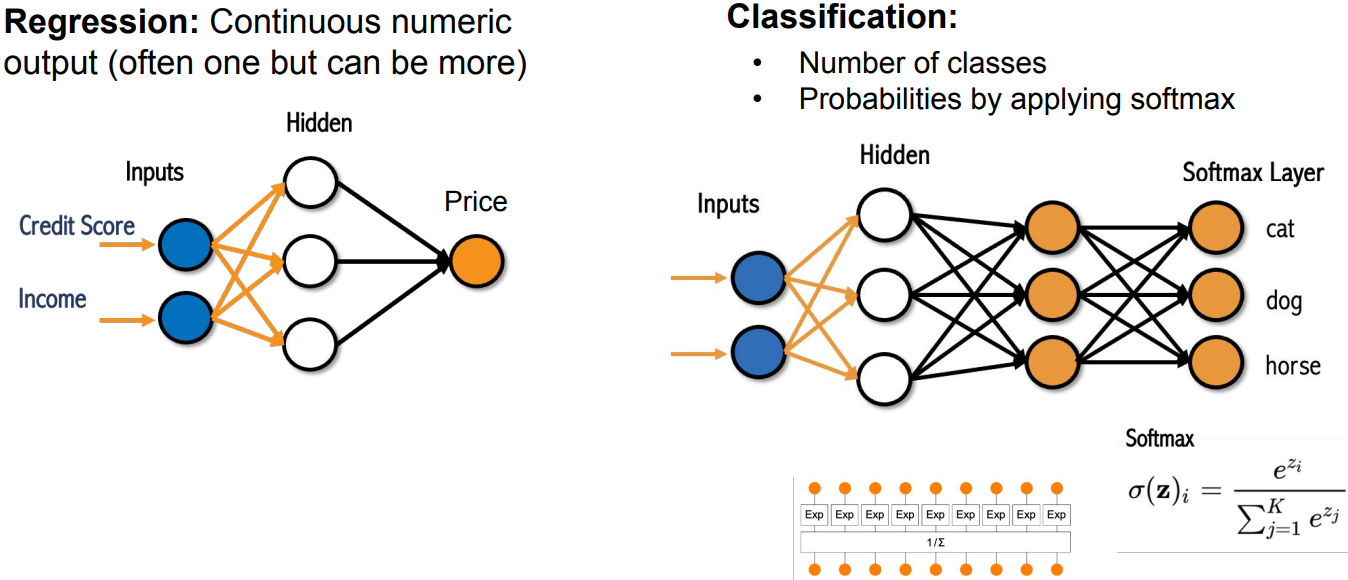
\includegraphics[width = \columnwidth]{figures/05/OutputNN.png}
\end{figure}
\subsubsection{Number of parameters}
Every connection(weights) + every Neuron(bias) = \# of parameters
